\documentclass[a4paper,12pt]{article}
\usepackage{color}
\usepackage{graphicx}
\usepackage{amsmath}

\begin{document}
\title{My First Document}
\author{Chandrashekhar Ghosh}
\date{\today}
\maketitle

\newpage
\pagenumbering{roman}
\tableofcontents
\newpage
\pagenumbering{arabic}

\section{Checkpoint 1 Introduction}
Hello ! I am a CSE student. This semester I am taking a course on \LaTeX, I am very exited.

\subsection{More about this course}
\label{Sec 1}

The formal name of this is Technical writing and presentation. In this course we will learn many things, but a significant part of this course is focused on \LaTeX\ because we will use it as a tool for other assignments of this course.

\subsection{Prerequisite of this course}
\label{Sec 2}

There is no prerequisite for this course. Anyone with will to learn can dive into this course.

\subsection{Summary}
Importance of \LaTeX\ see \ref{Sec 1}, for prerequisite see \ref{Sec 2}

\newpage

\section{Checkpoint 2 Typesetting Text}

\subsection{Font Effects}
Scientific Name of rice is \textit{Oryza sativa}.\\
Robert Frost famous quote \textsl{“\ Two roads diverged in a wood, and I – I took the road less traveled by”}.\\
\textsc{People's Republic of Bangladesh}\\
\textbf{In case of emergency call 999}.\\
\textsf{def square(a):\\ \indent return a*a }\\
\textrm{Rome didn't fall in a day}.\\
Scientific name of Mango is \underline{Mangifera} \underline{indica}.\\

\subsection{Coloured Text}
{\color{red}Apple}\\
{\color{yellow}Banana}\\
{\color{magenta}Pomegranate}\\

\subsection{Font Sizes}
Scientific classification of Bengal tiger.


Subspecies:\indent{\tiny \textit{P.t tigris}}


Species:\indent{\scriptsize \textit{p.tigris}}


Genus:\indent{\footnotesize \textit{Panthera}}


Subfamily:\indent{\small Pantherinae}


Family:\indent{\normalsize Felidae}


Suborder:\indent{\large Felifomia}


Order:\indent{\Large Carnivora}


Class:\indent{\LARGE Mammalia}


Phylum:\indent{\huge Chordata}

\newpage

\subsection{Lists}

Continents of the World.


\begin{enumerate}
    \item North America 
    \item South America
    \item Europe
    \item Africa 
    \item Asia
    \begin{itemize}
        \item North Asia
        \item Central Asia
        \item Western Asia
        \item South Asia
        \item East Asia
        \item Southeast Asia
    \end{itemize}
    \item Australia 
    \item Antarctica 
\end{enumerate}

\begin{itemize}
    \item[+] positive
    \item[-] negative
    \begin{itemize}
        \item[Fish] Hilsha.
        \item[Plant] Banyan.
    \end{itemize}
\end{itemize}

\subsection{Comments & Spacing}
\vspace{12pt}
\textsl{“\ It was the best of times,\\it was the worst of times,\\ it was the age of wisdom,\\it was the age of foolishness,\\ it was the epoch of belief,\\ it was the epoch of incredulity,\\it was the season of light,\\ it was the season of darkness,\\ it was the spring of hope,\\ it was the winter of despair.”}
% A Tale of Two Cities by Charles Dickens

\subsection{Special Characters}
\vspace{12pt}

The car \#1\textbackslash A costs \$ 120000 is sold at
a \~{}10\% profit.

\newpage

\section{Checkpoint 3 Tables}
\vspace{12pt}


\begin{tabular}{l|r|r}
     Item&Quantity&Price(\$) \\
     \hline
     Mangoes&10 Kg&20\\
     Apples&2 Kg&5\\
     Oranges& 1 Kg &5\\
\end{tabular}

\vspace{24pt}

\begin{tabular}{l|ccc}
    &\multicolumn{3}{c}{Year}\\
    \cline{2-4}
    City&2006&2007&2008\\
    \hline
    Dhaka & 242424 & 43535 & 55123\\
    New York & 100234 & 120432 & 110234\\
    Tokyo & 85673 & 90556 & 87234\\
\end{tabular}

\newpage

\section{Checkpoint 4 Figures}
\begin{figure}[h!]
    \centering
    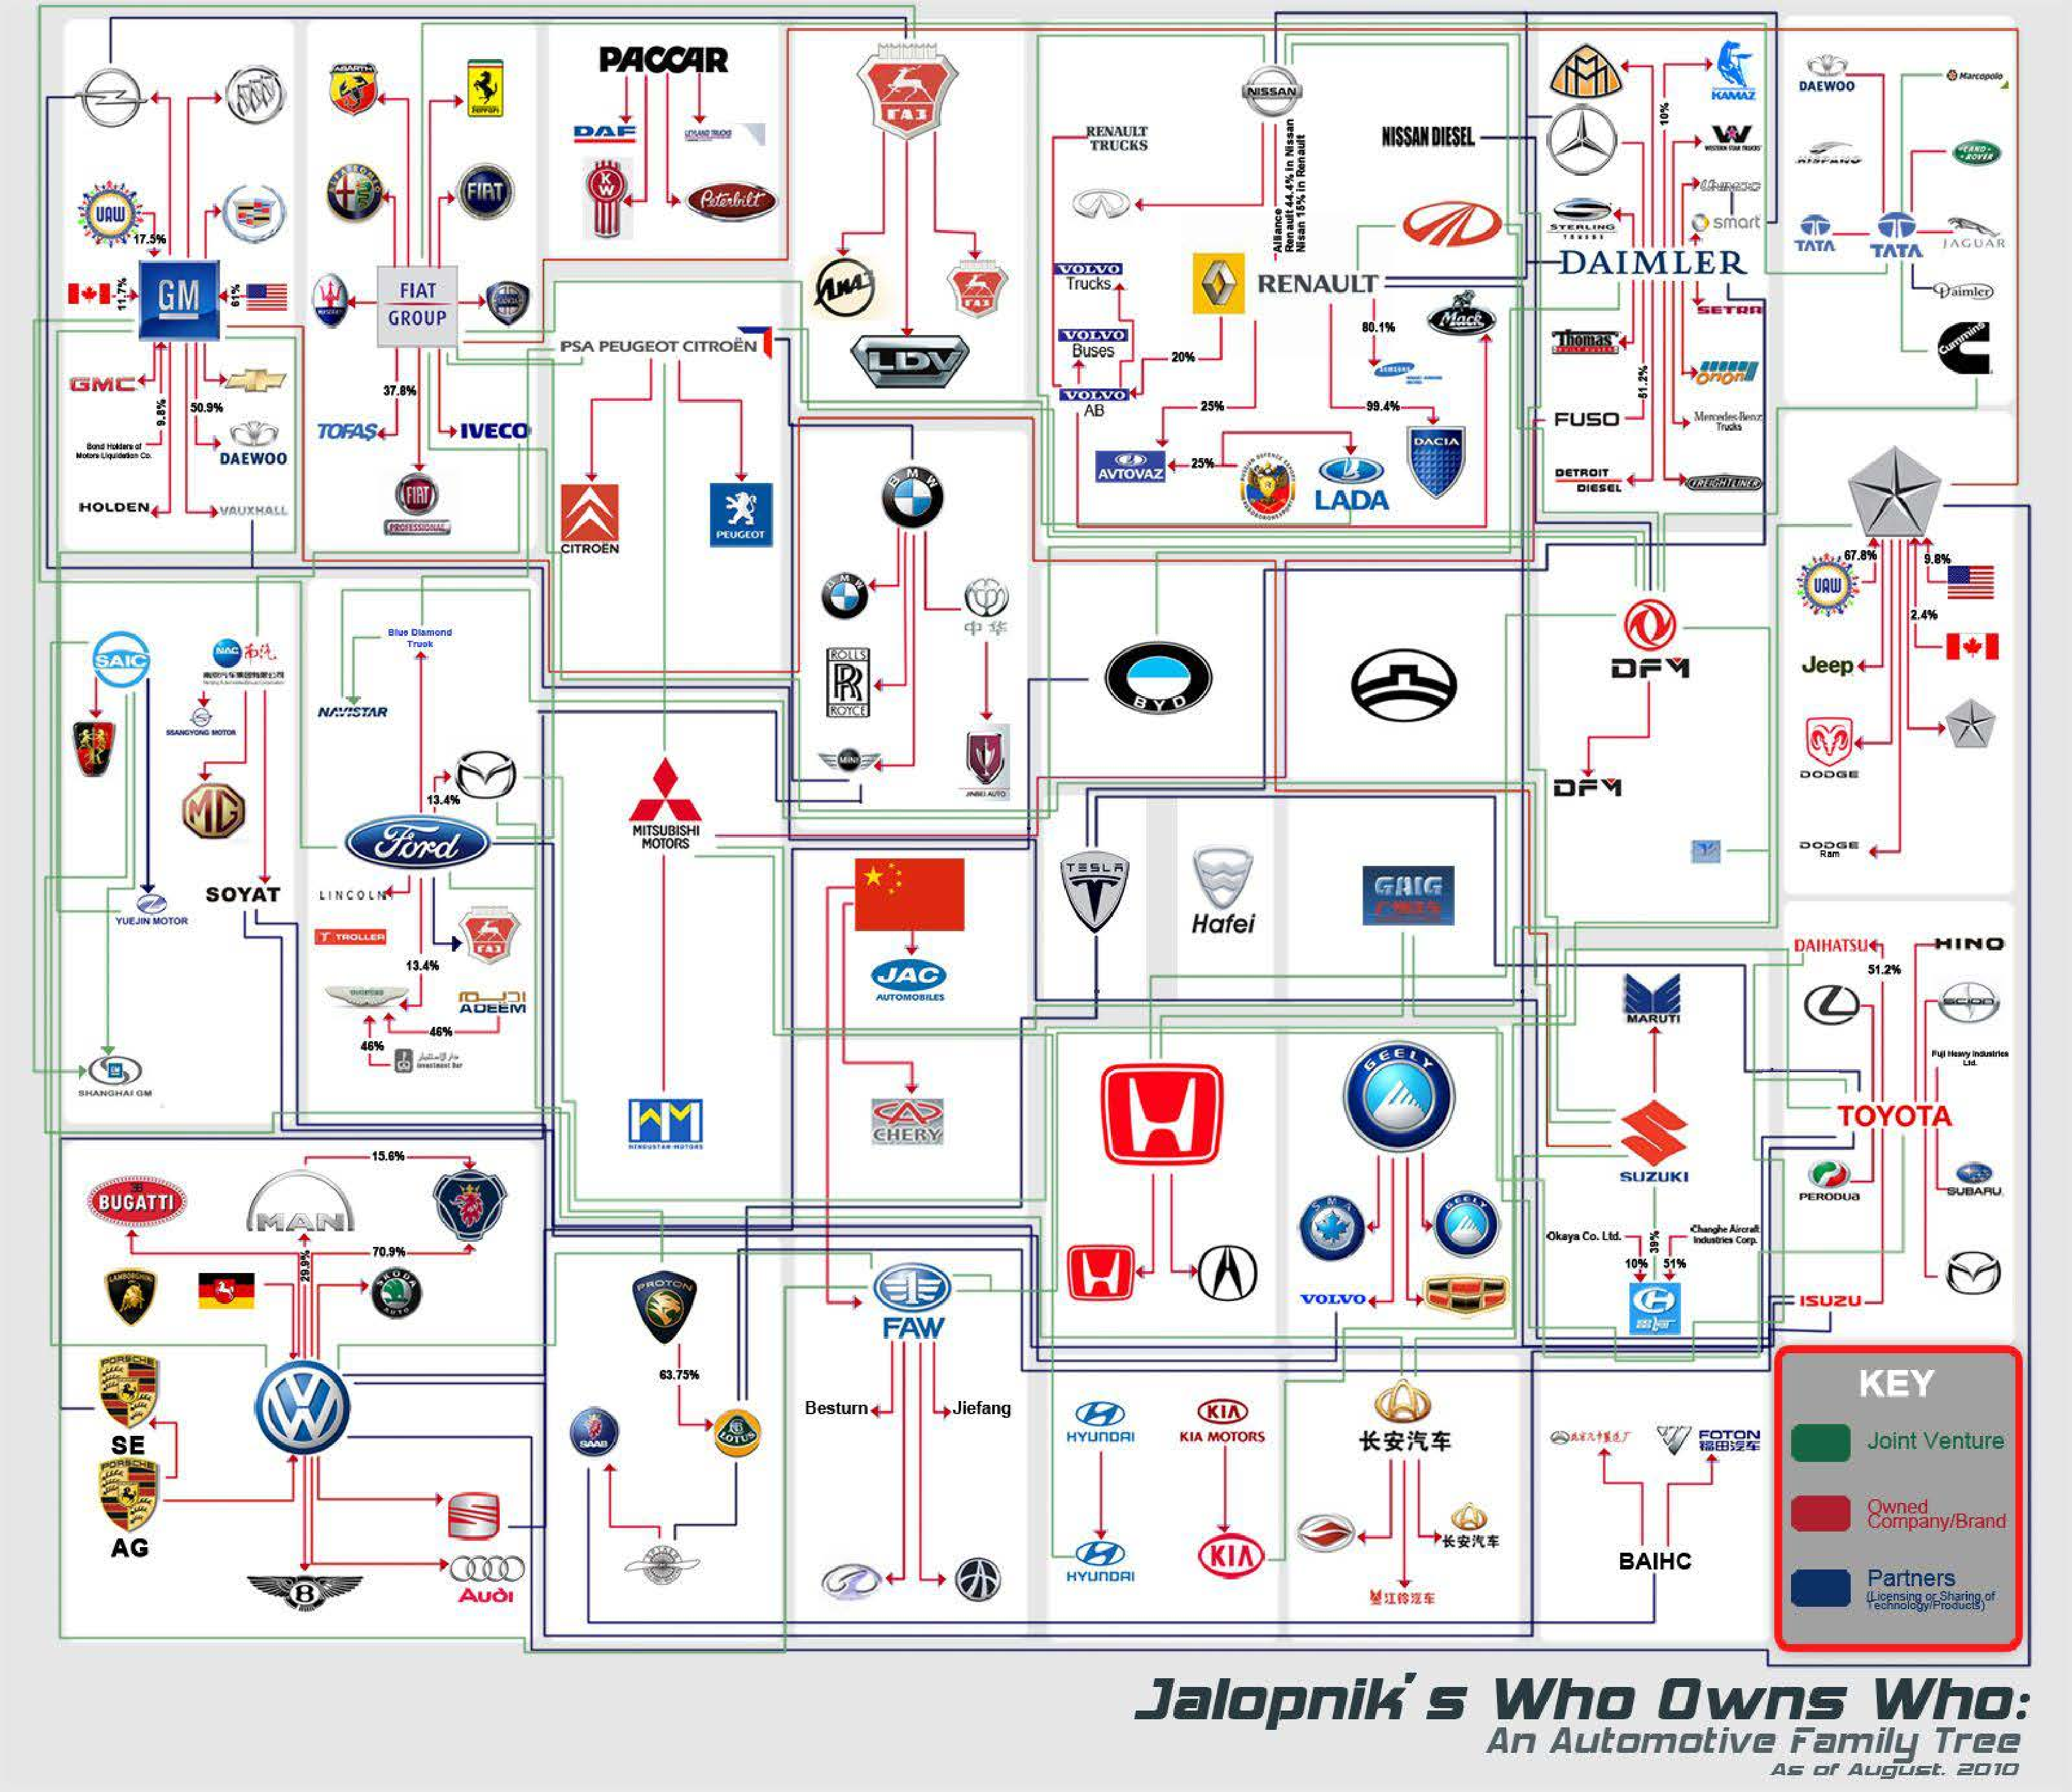
\includegraphics[scale =0.25]{image102.pdf}
    \caption{Car Companies}
\end{figure}

\newpage

\section{Checkpoint 5 Equations}
\vspace{12pt}

\begin{equation}
    e = mc^2
\end{equation}

\begin{equation}
    \pi = \frac{c}{d}
\end{equation}

\begin{equation}
    \frac{d}{dx}e^x = e^x
\end{equation}
\begin{equation}
    \frac{d}{dx} \int_0^\infty f(s)ds = f(x)
\end{equation}
 \begin{equation}
     f(x)=\sum_{i} = 0^\infty \frac{f^(i)(0)}{i!}x^i
 \end{equation}
 \begin{equation}
     x = \sqrt{\frac{x_i}{z}y}
 \end{equation}
\begin{equation}
\left[
\begin{matrix}
1 &2& 3& 4& 5\\
6 &7 & 8 & 9 & 10\\
11 & 12 & 13 & 14 & 15\\
16 & 17 & 18 & 19 & 20\\
21 & 22 & 23 & 24 &  25\\
\end{matrix}
\right]
\end{equation}

\newpage

\section{Checkpoint 6 Reference}
\vspace{12pt}
Let's cite some papers ...\\


1. paper number 1\cite{appice2020multi}\\


A computer vision book with very high citation.\cite{forsyth2011computer}\\


A paper on home networking.\cite{callaway2002home}\\


read about impact of parallel computing and distributed system in cybersecurity.\cite{kumar2005parallel}.\\


learn about deep learnign and cybersecurity.\cite{roopak2019deep}\\

\bibliographystyle{plain}
\bibliography{2017331102}




\end{document}